%!TEX root = main.tex
\setcounter{chapter}{6}
\setcounter{section}{1}
\setcounter{theorem}{0}
\setcounter{equation}{0}

\lectureheader{161}{Calculus I}{Volumes by cross sections}{\textit{Thomas' Calculus} \thesection}

\begin{definition}
The \textbf{volume} of a solid of integrable cross-sectional area $A(x)$ from $x=a$ to $x=b$ is
\begin{equation*}
V = \int_a^b A(x)\dee x.
\end{equation*}
\end{definition}
\begin{center}
\begin{tabular}{cc}
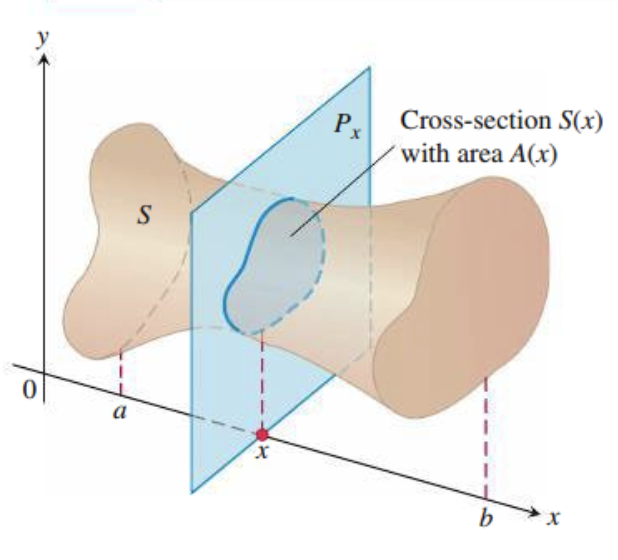
\includegraphics[width=3in]{img/cross-section} &
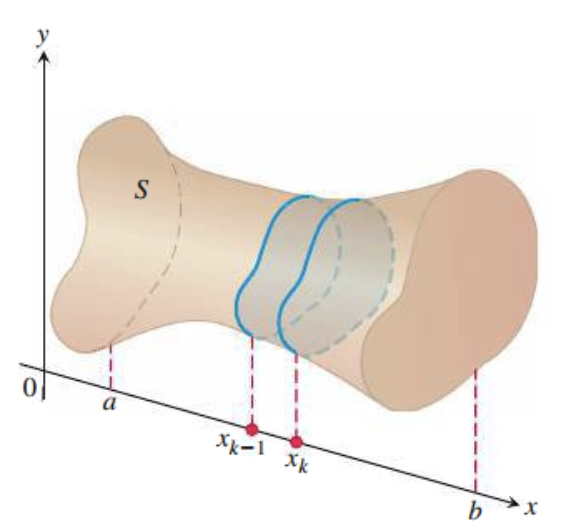
\includegraphics[width=3in]{img/differential_slab}
\end{tabular}
\end{center}
\begin{remark}
Sometimes the cross-sections that are perpendicular to the $y$-axis are more tractable.
If that is the case, then we may integrate with respect to $y$ instead.
\end{remark}

\newpage

\begin{example}
A pyramid $3$ \si{m} high has a square base that is $3$ \si{m} on a side.
The cross-section of the pyramid perpendicular to the altitude $x$ \si{m} down from the vertex is a square $x$ \si{m} on a side.
Find the volume of the pyramid.
\end{example}

\newpage

\begin{example}
A curved wedge is cut from a circular cylinder of radius $3$ by two planes.
One plane is perpendicular to the axis of the cylinder.
The second plane crosses the first at a 45\textdegree\ angle at the center of the cylinder.
Find the volume of the wedge.
\end{example}

\newpage

\begin{remark}
If we rotate a region in the $xy$-plane about an axis to create a solid, we call the object a \textbf{solid of revolution}.
If we slice the solid with planes that are perpendicular to the axis of revolution, then we find cross-sectional areas shaped like disks/washers.
\end{remark}

\begin{example}
The region between the curve $y=\sqrt x$ ($0\le x\le 4$), and the $x$-axis is revolved about the $x$-axis to generator a solid.
Find its volume.
\end{example}

\newpage

\begin{example}
The circle $x^2+y^2=r^2$ is rotated about the $x$-axis to generate a sphere.
Find its volume.
\end{example}

\newpage

\begin{example}
Find the volume of the solid generated by revolving the region bounded by $y=\sqrt x$ and the lines $y=1$, $x=4$ about the line $y=1$.
\end{example}

\newpage

\begin{example}
Find the volume of the solid generated by revolving the region between the $y$-axis and the curve 
\begin{equation*}
x=2/y\quad (1\le y\le 4)
\end{equation*}
about the $y$-axis.
\end{example}

\newpage

\begin{example}
Find the volume of the solid generated by revolving the region between the parabola $x=y^2+1$ and the line $x=3$ about the line $x=3$.
\end{example}

\newpage

\begin{example}
The region bounded by the curve $y=x^2+1$ and the line $y=-x+3$ is revolved about the $x$-axis.
Find the volume of the resulting solid of revolution.
\end{example}

\newpage

\begin{example}
The region in the first quadrant that is bounded by the parabola $y=x^2$ and the line $y=2x$ is revolved about the $y$-axis.  
Find the volume of the resulting solid of revolution.
\end{example}
